\chapter{Le problème} \label{chapPb}
\putminitoc
Depuis longtemps, l'entreprise avait un problème afin d'effectuer des tests d'intégrations, notamment pour les projets à destination de Ford. Les tests demandaient du temps et de l'argent à l'équipe en charge de ces tests. Ainsi, deux ans avant mon stage de M2, une solution a été trouvée : le développement d'un nouvelle outil, \textit{GreenT}.
	\section{Composant logiciel tiers}
	Étant donné la taille grandissante des programmes informatiques, il est de plus en plus rare qu'une seule et unique entité effectue le développement d'un logiciel.
	
	C'est ainsi que chez Continental, un certain nombre de composants des calculateurs ne sont pas développés en interne. Ce concept est appelé composant logiciel tiers, ou \textit{Third-Party Software}. 
	
	La principale difficulté de ce mode de fonctionnement est l'intégration, une spécification exhaustive est indispensable afin de pouvoir connecter les différentes interfaces du composant avec le reste du projet. 
	
	C'est avec ces contraintes que travaillent plusieurs équipes chez Continental et notamment l'équipe en charge du développement des différents logiciels de contrôle moteur à destination de Ford.
	
	\section{Les tests du << plugin >> Ford}\label{plugin}
	Comme dit précédemment, Continental ne développe pas l'intégralité du logiciel pour Ford, une partie étant fournie par le client sous forme de << plugin >>. Ce plugin est un fichier binaire qui est chargé directement dans la mémoire flash de l'ECU sans que Continental n'ait accès au code source. Seule une description des interfaces est fournie. Le \textit{plugin} est supposé correct, et le tester n'est pas de notre ressort. Cependant, celui-ci va être interfacé avec les logiciels Continental : il est indispensable de vérifier que les deux parties fonctionnent ensemble lors de l'intégration.
	\begin{figure}[H]
		\centering
		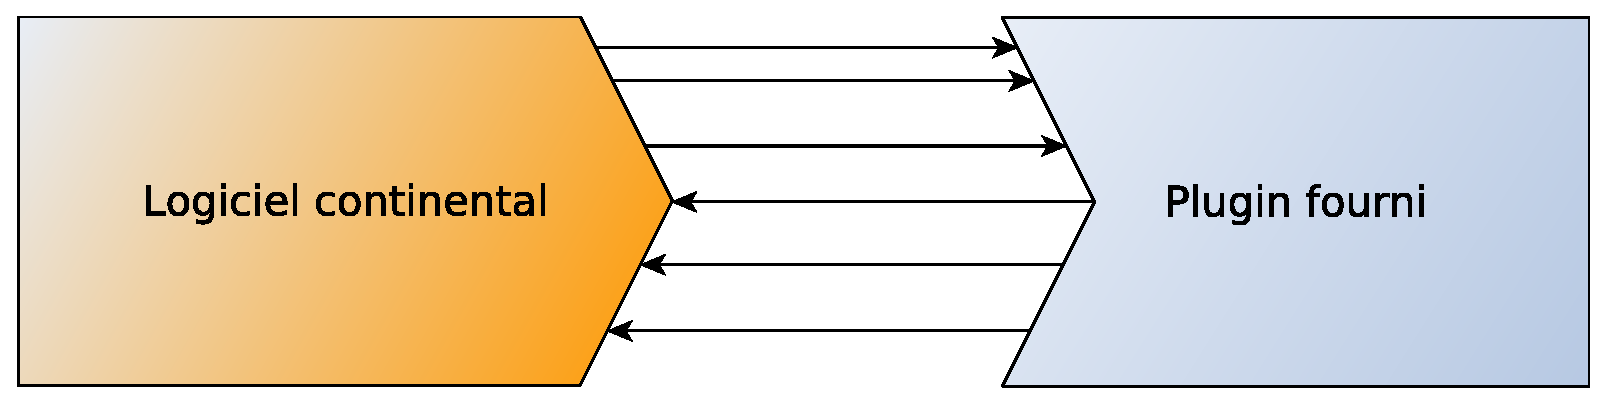
\includegraphics[width=8.0cm]{contents/images/plugin.eps}
		\caption{Interfaces du plugin avec le logiciel de Continental}
		\label{fig:plugin}	
	\end{figure}
	
	Le fichier de spécification est un fichier Excel, fourni par le client. Ce fichier, appelé \textit{Walkthrough}\footnote{Ce fichier est expliqué plus en détail section \ref{wt}}, 
	contient la liste de toutes les variables du plugin avec toutes leur spécifications. Il contient
	environ 1200 variables différentes. 
	
	Il est impensable de tester le fonctionnement d'autant de paramètres manuellement. Ainsi l'équipe en
	charge de tester cette intégration effectue des tests de différence d'une version à l'autre : seules les variables ayant pu être impactées par une \textit{release} seront testées, il est supposé que le fonctionnement des autres variables reste inchangé. Ce type de test est appelé \textit{Delta Test}.
	
	\vspace{20px}
	Deux problèmes se posent à cette méthode : 
	\begin{description}
		\item[La fiabilité des tests manuels] Le test des seules différences ne permet pas nécessairement de détecter tous les problèmes. De plus, une tâche répétitive peut entrainer des erreurs humaines.
		\item[Le temps de tests] Même en ne testant qu'une partie des variables, cela prend un temps considérable, il faut compter environ une semaine.\newline
			Or, les tests s'effectuent sur les bancs de tests comme expliqué section \ref{wb}, ces équipements permettent de simuler un environnement véhicule du contrôleur moteur comme
			l'utilisation de la clé de démarrage, la tension de la batterie, la vitesse de rotation du moteur, \ldots Ceux-ci sont peu
			nombreux dans l'entreprise en raison de leur coût, leur disponibilité est donc compliquée. Il serait intéressant de pouvoir lancer
			des tests automatisés durant la nuit par exemple afin d'optimiser au maximum leur utilisation.
	\end{description}
	
\newpage
	\section{La solution : \textit{GreenT}}
	Pour répondre aux besoins de l'équipe Ford, une solution a été pensée en étudiant leurs besoins : le développement de \textit{GreenT}
	\begin{remarque}
		Le nom de \textit{GreenT} provient de la contraction de \textit{Green} et \textit{Test}.
		
		En effet, un test est signalé correct si celui-ci est vert, or le but de notre plateforme est d'automatiser des tests et qu'à la fin de l'exécution, tout ceux-ci soient verts.
	\end{remarque}
	
	\subsection{Les tests d'intégration du plugin Ford}
		Depuis Janvier dernier, GreenT est sorti en version 1.0, ainsi cette solution permet de tester le plugin pour les projets Ford facilement et de façon efficace.
		
		 Pour cela, un testeur de l'équipe à ajouté des colonnes dans le document \textit{Walkthrough}, afin de spécifier la manière de tester les variables. L'outil est capable d'analyser le document \textit{Walkthrough}, et de générer les tests automatiques. Il est ensuite possible de planifier son exécution, celle-ci prendre deux heures pour 270 tests. Une fois l'exécution terminée, le testeur a tous les résultats de ces tests, il peut ainsi regarder les rapports détaillés afin de corriger les éventuels problèmes.
	
	Ces tests s'effectuent sur des variables enregistrées lors de stimulation de l'ECU, afin de vérifier que celui-ci réagit de façon approprié.

	Cet outil permettra ensuite de tester facilement la dizaine de projets Ford, et une fois le test d'une variable spécifié, il n'est plus nécessaire de le réécrire. À chaque nouvelle version du logiciel, ou \textit{release}, il suffit de relancer les tests : l'équipe n'a à faire le travail qu'une fois en début de projet, ensuite la réutilisation sera possible, les projets seront testés plus rapidement, plus efficacement, et plus souvent.

	\subsection{Les autres projets}
	À court terme, cet outil pourrait être utilisée pour les projets d'autres clients tel que Renault, afin d'effectuer là aussi des tests d'intégration. Il était donc nécessaire de concevoir un outil qui puisse évoluer facilement, et puisse avoir un fichier de spécification en entrée qui soit légèrement différent d'un client à l'autre.
	
	Afin que notre outil puisse fonctionner sur le maximum de projets différents, et qu'il puisse également servir à effectuer des tests d'intégration indépendamment du cadre d'un \textit{third party software}, j'ai mis en place un fichier de spécification en entrée totalement générique. Plus d'information sur ce fichier section \ref{gttestplan}.
	
	Renault à cependant des besoins légèrement différents de ceux de Ford, pouvoir exprimer un test en fonction de variables ECU, tel que Ford, mais également de symboles HiL. Une nouvelle fonctionnalité est donc en développement comme présenté section \ref{synchro}.
%	En effet, les autres clients peuvent aussi fournir une partie du logiciel, avec un document de spécification des variables, celui-ci ne serait pas totalement identique, mais il s'en approchera.

%	Il est également envisageable que la plateforme soit utilisée pour des tests d'intégration en interne, indépendamment des spécifications fournies par un client externe à Continental.
%	\newpage
%	\subsection{L'utilisation de \textit{GreenT} comme une bibliothèque}
%	Une autre approche de notre plateforme, serait de s'en servir pour écrire facilement des tests en Java, de façon plus efficace et plus robuste qu'avec la TA3 : notre plateforme doit donc également fonctionner comme une bibliothèque sans utilisation de générateur ou de parser, pour que le testeur puisse effectuer un test rapide. 
%
%	Celui-ci apprendra à se servir de la plateforme, écrira en règle générale des tests assez courts et moins complexes que ceux que nous générerons, ceux-ci doivent être faciles à écrire.
%
%\begin{remarque}
%	\textit{GreenT} fonctionne avec un modèle client-serveur comme cela sera détaillé chapitre \ref{chapGreent}.
%	
%	 Afin de commencer à effectuer une livraison dans l'optique de l'utilisation de \textit{GreenT} en tant que bibliothèque, nous avons déjà fourni les premières versions des serveurs à plusieurs personnes. Celles-ci utilisent nos serveurs en effectuant des scripts simples depuis un an sans problème.
%\end{remarque}